% =====================================================================
%  PIM IV — UrbanoAcessível S.A.  ·  Relatório acadêmico (ABNT / UNIP)
%  Compilar: pdflatex relatorio.tex (duas vezes, para o sumário)
% =====================================================================
\documentclass[12pt,a4paper,oneside]{report}

\usepackage[T1]{fontenc}
\usepackage[utf8]{inputenc}
\usepackage[english]{babel}
\babelprovide[import,main]{portuguese}
\usepackage{mathptmx}                       % Times New Roman
\usepackage[a4paper,top=3cm,left=3cm,bottom=2cm,right=2cm,headheight=14pt,headsep=0.6cm]{geometry}
\usepackage{setspace}
\usepackage{indentfirst}
\usepackage{graphicx}
\usepackage{float}
\usepackage{array,tabularx,longtable,multirow}
\usepackage[table]{xcolor}
\usepackage{caption}
\usepackage{titlesec}
\usepackage{tocloft}
\usepackage{fancyhdr}
\usepackage{enumitem}
\usepackage{listings}
\usepackage[hidelinks,bookmarksnumbered,pdfusetitle]{hyperref}

\hypersetup{
  pdftitle={Sistema Corporativo de Gestão da Frota, Manutenção Preventiva e Chamados de Acessibilidade},
  pdfauthor={Alfredo Allan Teixeira Sousa},
  pdfsubject={PIM IV - UrbanoAcessível S.A.},
  pdfkeywords={engenharia de software, banco de dados, linguagem C, acessibilidade, IoT}
}

% ---------------------------------------------------- espaçamento e parágrafo
\onehalfspacing
\setlength{\parindent}{1.5cm}
\setlength{\parskip}{0pt}
\frenchspacing
\sloppy

% ---------------------------------------------------- títulos (NBR 6024)
\renewcommand{\chaptername}{}
\titleformat{\chapter}[hang]{\normalfont\normalsize\bfseries}{\thechapter}{0.6em}{\MakeUppercase}
\titlespacing*{\chapter}{0pt}{0pt}{1.5\baselineskip}
\titleformat{\section}[hang]{\normalfont\normalsize\bfseries}{\thesection}{0.6em}{}
\titlespacing*{\section}{0pt}{1.5\baselineskip}{1\baselineskip}
\titleformat{\subsection}[hang]{\normalfont\normalsize}{\thesubsection}{0.6em}{}
\titlespacing*{\subsection}{0pt}{1.5\baselineskip}{1\baselineskip}
\setcounter{secnumdepth}{3}
\setcounter{tocdepth}{2}

% títulos sem indicativo numérico, centralizados (resumo, sumário, referências...)
\newcommand{\titulocentral}[1]{%
  \begin{center}\textbf{\MakeUppercase{#1}}\end{center}\vspace{0.8\baselineskip}}

% ---------------------------------------------------- sumário
\renewcommand{\contentsname}{Sumário}
\renewcommand{\cftchapfont}{\bfseries}
\renewcommand{\cftchappagefont}{\bfseries}
\renewcommand{\cftsecfont}{\bfseries}\renewcommand{\cftsecpagefont}{\bfseries}
\renewcommand{\cftchapleader}{\bfseries\cftdotfill{\cftdotsep}}
\renewcommand{\cftchapaftersnum}{}
\setlength{\cftbeforechapskip}{4pt}
\setlength{\cftchapindent}{0pt}
\setlength{\cftsecindent}{0pt}
\setlength{\cftsubsecindent}{0pt}
\setlength{\cftchapnumwidth}{2em}
\setlength{\cftsecnumwidth}{2.6em}
\setlength{\cftsubsecnumwidth}{3.4em}
\renewcommand{\cfttoctitlefont}{\hfill\bfseries\MakeUppercase}
\renewcommand{\cftaftertoctitle}{\hfill}
\renewcommand{\cftloftitlefont}{\hfill\bfseries\MakeUppercase}
\renewcommand{\cftafterloftitle}{\hfill}
\setlength{\cftbeforetoctitleskip}{0pt}
\setlength{\cftbeforeloftitleskip}{0pt}
\setlength{\cftfignumwidth}{6.2em}
\setlength{\cftfigindent}{0pt}

% ---------------------------------------------------- legendas ABNT
\captionsetup{font={small},labelsep=endash,justification=centering,skip=4pt,singlelinecheck=false}
\DeclareCaptionListFormat{fig}{Figura~#2~--}
\DeclareCaptionListFormat{qd}{Quadro~#2~--}
\captionsetup[figure]{name=Figura,position=above,listformat=fig}
\captionsetup[table]{position=above}
\DeclareCaptionType[fileext=loq,placement=H]{quadro}[Quadro][Lista de quadros]
\captionsetup[quadro]{position=above,listformat=qd}
\newcommand{\fonte}[1]{\par\vspace{2pt}{\small Fonte: #1}\par}
\renewcommand{\thefigure}{\arabic{figure}}
\renewcommand{\thequadro}{\arabic{quadro}}


% ---------------------------------------------------- código-fonte
\definecolor{cinza}{gray}{0.45}
\definecolor{fundo}{gray}{0.96}
\renewcommand{\lstlistingname}{Código}
\lstset{
  basicstyle=\ttfamily\footnotesize\linespread{1}\selectfont,
  keywordstyle=\bfseries,
  commentstyle=\itshape\color{cinza},
  stringstyle=\color{black},
  backgroundcolor=\color{fundo},
  frame=single, rulecolor=\color{gray!60},
  breaklines=true, breakatwhitespace=false, columns=fullflexible, keepspaces=true,
  showstringspaces=false, tabsize=4, xleftmargin=4pt, xrightmargin=4pt,
  numbers=left, numberstyle=\tiny\color{cinza}, numbersep=6pt,
  captionpos=t, abovecaptionskip=4pt, belowcaptionskip=4pt,
  extendedchars=true,
  literate={á}{{\'a}}1 {é}{{\'e}}1 {í}{{\'i}}1 {ó}{{\'o}}1 {ú}{{\'u}}1 {ã}{{\~a}}1 {õ}{{\~o}}1
           {ç}{{\c c}}1 {â}{{\^a}}1 {ê}{{\^e}}1 {ô}{{\^o}}1 {Ç}{{\c C}}1 {Á}{{\'A}}1 {É}{{\'E}}1 {Ã}{{\~A}}1
}
\lstdefinelanguage{JSON}{morestring=[b]", sensitive=true, morekeywords={true,false,null}}
\lstdefinelanguage{SQLm}[]{SQL}{morekeywords={AUTO_INCREMENT,TIMESTAMP,DATETIME,TEXT,INNER,LEFT,COALESCE,ROUND,START,TRANSACTION,COMMIT,REFERENCES,CHECK,INDEX}}

% ---------------------------------------------------- cabeçalho (página no canto superior direito)
\pagestyle{fancy}
\fancyhf{}
\fancyhead[R]{\small\thepage}
\renewcommand{\headrulewidth}{0pt}
\fancypagestyle{plain}{\fancyhf{}\fancyhead[R]{\small\thepage}\renewcommand{\headrulewidth}{0pt}}

\setlist{itemsep=0pt,topsep=4pt,leftmargin=1.5cm}


% ---------------------------------------------------- citações autor-data (NBR 10520)
\newcommand{\defref}[4]{\expandafter\def\csname rA@#1\endcsname{#2}%
  \expandafter\def\csname rB@#1\endcsname{#3}\expandafter\def\csname rY@#1\endcsname{#4}}
\renewcommand{\cite}[1]{(\csname rA@#1\endcsname, \csname rY@#1\endcsname)}
\newcommand{\citeonline}[1]{\csname rB@#1\endcsname{} (\csname rY@#1\endcsname)}
\defref{cf88}{BRASIL}{Brasil}{1988}
\defref{lbi}{BRASIL}{Brasil}{2015}
\defref{lgpd}{BRASIL}{Brasil}{2018}
\defref{wcag}{W3C}{W3C}{2018}
\defref{tanenbaum}{TANENBAUM; WETHERALL}{Tanenbaum e Wetherall}{2011}
\defref{gil}{GIL}{Gil}{2017}
\defref{lakatos}{LAKATOS; MARCONI}{Lakatos e Marconi}{2017}
\defref{pressman}{PRESSMAN; MAXIM}{Pressman e Maxim}{2016}
\defref{scrum}{SCHWABER; SUTHERLAND}{Schwaber e Sutherland}{2020}
\defref{beck}{BECK}{Beck}{2004}
\defref{sommerville}{SOMMERVILLE}{Sommerville}{2018}
\defref{fowler}{FOWLER}{Fowler}{2005}
\defref{sadalage}{SADALAGE; FOWLER}{Sadalage e Fowler}{2013}
\defref{silberschatz}{SILBERSCHATZ; KORTH; SUDARSHAN}{Silberschatz, Korth e Sudarshan}{2012}
\defref{elmasri}{ELMASRI; NAVATHE}{Elmasri e Navathe}{2018}
\defref{mongodb}{MONGODB, INC.}{MongoDB, Inc.}{2026}
\defref{kernighan}{KERNIGHAN; RITCHIE}{Kernighan e Ritchie}{1989}
\defref{iso9899}{INTERNATIONAL ORGANIZATION FOR STANDARDIZATION}{International Organization for Standardization}{1999}

\usepackage{chngcntr}
\counterwithout{figure}{chapter}
\counterwithout{quadro}{chapter}
\usepackage{etoolbox}
\makeatletter
\patchcmd{\@chapter}{\addtocontents{lof}{\protect\addvspace{10\p@}}}{}{}{}
\patchcmd{\@chapter}{\addtocontents{lot}{\protect\addvspace{10\p@}}}{}{}{}
\makeatother
\AtBeginDocument{\counterwithout{lstlisting}{chapter}\renewcommand{\thelstlisting}{\arabic{lstlisting}}}

% ---------------------------------------------------- dados do trabalho (edite aqui)
\newcommand{\instituicao}{UNIVERSIDADE PAULISTA -- UNIP EAD}
\newcommand{\polo}{POLO [NOME DO POLO]}
\newcommand{\curso}{CURSO SUPERIOR DE TECNOLOGIA EM ANÁLISE E DESENVOLVIMENTO DE SISTEMAS}
\newcommand{\autores}{%
  ALFREDO ALLAN TEIXEIRA SOUSA\\RA: 2636870}
\newcommand{\titulo}{URBANOACESSÍVEL S.A.: SISTEMA CORPORATIVO DE GESTÃO DA FROTA, MANUTENÇÃO PREVENTIVA E CHAMADOS DE ACESSIBILIDADE}
\newcommand{\subtitulo}{Projeto Integrado Multidisciplinar IV}
\newcommand{\orientador}{Prof.(ª) Nome do(a) Orientador(a)}
\newcommand{\cidade}{SÃO PAULO}
\newcommand{\ano}{2026}

\begin{document}

% ===================================================================== CAPA
\pdfbookmark[0]{Capa}{capa}
\begin{titlepage}
  \thispagestyle{empty}
  \centering\bfseries
  \instituicao\\[2pt]\curso\\[2pt]\polo\par
  \vspace{2.5cm}
  \normalfont\autores\par
  \vfill
  \bfseries\titulo\par
  \vspace{0.5cm}\normalfont\subtitulo\par
  \vfill
  \bfseries\cidade\\\ano
\end{titlepage}

% ===================================================================== FOLHA DE ROSTO
\setcounter{page}{1}
\thispagestyle{empty}
\pdfbookmark[0]{Folha de rosto}{rosto}
\begin{center}
  \autores\par
  \vspace{4cm}
  \textbf{\titulo}\par
  \vspace{2cm}
\end{center}
\begin{flushright}
  \begin{minipage}{0.5\textwidth}
    \singlespacing\small
    Projeto Integrado Multidisciplinar IV apresentado ao Curso Superior de Tecnologia em Análise e
    Desenvolvimento de Sistemas da Universidade Paulista -- UNIP, na modalidade de Educação a Distância, como requisito parcial para
    aprovação no semestre letivo, integrando as disciplinas de Engenharia de Software Ágil,
    Banco de Dados e Linguagem e Técnicas de Programação.\par\vspace{0.8cm}
    Orientador(a): \orientador
  \end{minipage}
\end{flushright}
\vfill
\begin{center}\textbf{\cidade\\\ano}\end{center}
\clearpage

% ===================================================================== RESUMO
\thispagestyle{empty}
\pdfbookmark[0]{Resumo}{resumo}
\titulocentral{Resumo}
\noindent
Este trabalho apresenta o desenvolvimento do Sistema Corporativo de Gestão da Frota, Manutenção
Preventiva e Chamados de Acessibilidade da UrbanoAcessível Soluções em Mobilidade e Tecnologia S.A.,
empresa fictícia que integra sensores IoT embarcados em ônibus urbanos a uma arquitetura em nuvem
para monitorar elevadores hidráulicos, rampas e assentos reservados. Dando continuidade ao PIM III,
que definiu a infraestrutura de redes segmentada em VLANs, o broker MQTT na nuvem e os requisitos de
acessibilidade e proteção de dados, o PIM IV concentra-se no software que transforma a telemetria em
ação. Adotou-se o processo ágil Scrum, com práticas da Programação Extrema, em três sprints. Foram
levantados oito requisitos funcionais e cinco não funcionais, modelados em diagramas UML de casos de
uso, de classes e de atividades. O armazenamento seguiu a persistência poliglota: um banco relacional
normalizado até a terceira forma normal guarda veículos, mecânicos e ordens de serviço, com integridade
referencial garantida por chaves estrangeiras, enquanto uma coleção de documentos no MongoDB absorve os
registros de telemetria de alta frequência. O núcleo operacional foi implementado em linguagem C,
dividido em seis módulos, com menu interativo, leitura segura de entradas, controle de acesso por perfil
e persistência em arquivos de texto gravados de forma atômica. O programa abre automaticamente uma ordem
de serviço quando um sensor reporta falha no elevador e calcula o percentual da frota com
acessibilidade plenamente ativa. Os testes confirmaram a recuperação dos dados após reinicialização, a
recusa de ordens para veículos inexistentes e a compilação sem avisos com GCC. Conclui-se que a solução
atende aos requisitos propostos e oferece ao poder público um indicador objetivo para fiscalizar o
direito de ir e vir das pessoas com deficiência.

\vspace{\baselineskip}
\noindent\textbf{Palavras-chave:} engenharia de software; banco de dados; linguagem C; Internet das
Coisas; acessibilidade.
\clearpage

% ===================================================================== ABSTRACT
\thispagestyle{empty}
\pdfbookmark[0]{Abstract}{abstract}
\begin{otherlanguage}{english}
\titulocentral{Abstract}
\noindent
This work presents the development of the Corporate Fleet Management, Preventive Maintenance and
Accessibility Ticketing System of UrbanoAcessível Soluções em Mobilidade e Tecnologia S.A., a fictitious
company that connects IoT sensors installed on city buses to a cloud architecture in order to monitor
hydraulic lifts, ramps and priority seats. Building on PIM III, which defined a VLAN-segmented network,
a cloud MQTT broker and the accessibility and data protection requirements, PIM IV focuses on the
software that turns telemetry into action. The Scrum agile process, combined with Extreme Programming
practices, was carried out in three sprints. Eight functional and five non-functional requirements were
elicited and modeled with UML use case, class and activity diagrams. Storage follows polyglot
persistence: a relational database normalized to third normal form keeps vehicles, mechanics and work
orders, with referential integrity enforced by foreign keys, while a MongoDB document collection absorbs
high-frequency telemetry records. The operational core was implemented in the C language, split into six
modules, with an interactive menu, safe input handling, role-based access control and persistence in text
files written atomically. The program automatically opens a work order when a sensor reports a lift
failure and computes the share of the fleet with fully working accessibility. Tests confirmed data
recovery after restart, rejection of work orders for non-existent vehicles and warning-free compilation
with GCC. The solution meets the proposed requirements and gives public authorities an objective
indicator to oversee the right to mobility of people with disabilities.

\vspace{\baselineskip}
\noindent\textbf{Keywords:} software engineering; databases; C language; Internet of Things;
accessibility.
\end{otherlanguage}
\clearpage

% ===================================================================== LISTAS
\thispagestyle{empty}
\pdfbookmark[0]{Lista de figuras}{lof}
\renewcommand{\listfigurename}{Lista de figuras}\renewcommand{\figurename}{Figura}
{\singlespacing\listoffigures}
\thispagestyle{empty}
\clearpage
\thispagestyle{empty}
\pdfbookmark[0]{Lista de quadros}{loq}
{\singlespacing\listofquadros}
\thispagestyle{empty}
\clearpage

% ===================================================================== SUMÁRIO
\pdfbookmark[0]{Sumário}{sumario}
\thispagestyle{empty}
\renewcommand{\contentsname}{Sumário}{\singlespacing\tableofcontents}
\thispagestyle{empty}
\clearpage

% =====================================================================
%  ELEMENTOS TEXTUAIS
% =====================================================================
\chapter{INTRODUÇÃO}

O transporte público coletivo é, para grande parte da população brasileira, a única forma de acesso ao
trabalho, à escola e aos serviços de saúde. Para pessoas com deficiência, idosos, gestantes e pessoas com
mobilidade reduzida, porém, o embarque depende de equipamentos que falham com frequência: o elevador
hidráulico que não desce, a rampa que trava, o assento reservado ocupado sem sinalização. Quando a falha
só é descoberta no ponto de ônibus, o passageiro perde a viagem e o direito de ir e vir, assegurado pelo
art. 5º, inciso XV, da Constituição Federal \cite{cf88}, deixa de ser exercido na prática.

A UrbanoAcessível Soluções em Mobilidade e Tecnologia S.A. é uma empresa fictícia do segmento de cidades
inteligentes, criada ao longo dos Projetos Integrados Multidisciplinares do curso. Seus clientes são
secretarias municipais de transporte, órgãos gestores de trânsito e concessionárias de transporte
coletivo; seus usuários finais são os passageiros que dependem de recursos de acessibilidade.

\section{Continuidade em relação ao PIM III}

No PIM III foi construída a base de infraestrutura da empresa. A rede corporativa adotou uma topologia
hierárquica em estrela estendida, com roteador de borda Cisco 2911, núcleo Layer 3 Cisco 3560-24PS e
switches de acesso Cisco 2960-24TT, segmentada em quatro VLANs no bloco 10.0.0.0/16, conforme a
Figura~\ref{fig:topologia}. A VLAN 30 concentra os gateways de telemetria da frota, e a VLAN 40 isola a
rede de visitantes por meio de lista de controle de acesso. A interligação entre switches usa enlaces
tronco IEEE 802.1Q, e o roteamento entre VLANs é feito por interfaces virtuais (SVI) no núcleo, prática
descrita por \citeonline{tanenbaum}.

\begin{figure}[H]
  \centering
  \caption{Topologia de rede hierárquica definida no PIM III}\label{fig:topologia}
  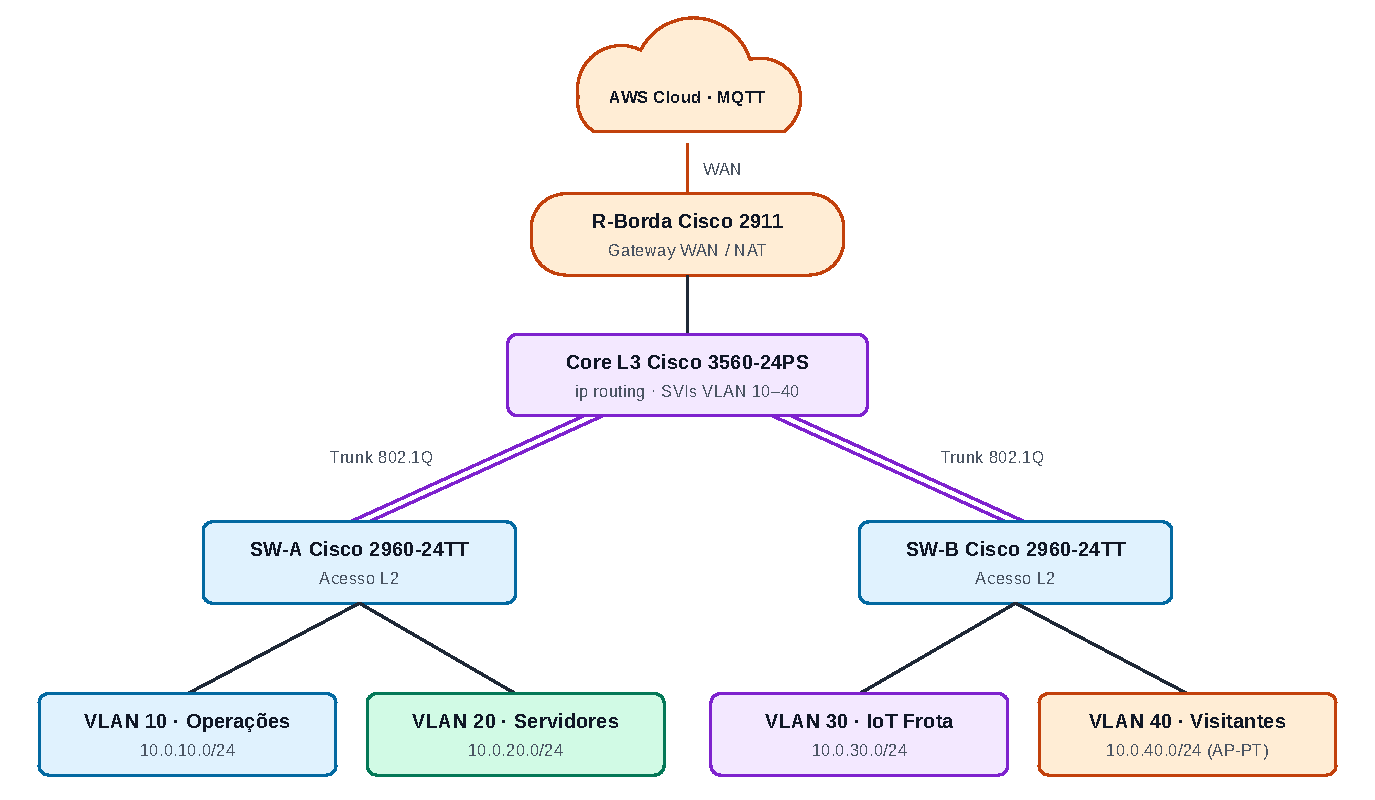
\includegraphics[width=0.82\textwidth]{fig/tp.pdf}
  \fonte{Elaborado pelo autor (2026).}
\end{figure}

Na nuvem, um broker MQTT recebe pela rede móvel 4G/5G as mensagens enviadas pelos ônibus em trânsito,
com o estado do elevador, as coordenadas GPS e a lotação. Microsserviços de ingestão, processamento de
alertas e API REST, protegidos por balanceador de carga, escalonamento automático e TLS 1.3 com
certificados X.509 por dispositivo, completam a arquitetura. O PIM III também estabeleceu os requisitos
de acessibilidade digital segundo a WCAG 2.1 nível AA \cite{wcag} e de proteção de dados segundo a Lei
Geral de Proteção de Dados Pessoais \cite{lgpd}.

O PIM III, portanto, resolveu \emph{como o dado chega}. Faltava responder \emph{o que fazer com ele}: quem
é avisado quando um elevador quebra, como se agenda o conserto, como se prova à prefeitura quantos ônibus
estão de fato acessíveis. Essa é a matéria do PIM IV.

\section{Objetivos}

O objetivo geral deste trabalho é desenvolver o Sistema Corporativo de Gestão da Frota, Manutenção
Preventiva e Chamados de Acessibilidade da UrbanoAcessível S.A., integrando engenharia de software ágil,
modelagem de banco de dados relacional e não relacional e programação estruturada em linguagem C com
persistência em arquivos.

Os objetivos específicos são:
\begin{enumerate}[label=\alph*)]
  \item levantar e documentar os requisitos funcionais e não funcionais do sistema;
  \item planejar o desenvolvimento em sprints, com backlog priorizado em histórias de usuário;
  \item modelar o sistema com diagramas UML de casos de uso, de classes e de atividades;
  \item projetar o banco relacional normalizado e a coleção NoSQL para a telemetria;
  \item implementar em C o núcleo operacional, com persistência em disco e controle de acesso;
  \item testar o programa e verificar o atendimento a cada requisito.
\end{enumerate}

\section{Justificativa}

A Lei Brasileira de Inclusão \cite{lbi} assegura à pessoa com deficiência o direito ao transporte e à
mobilidade em igualdade de oportunidades com as demais pessoas. Fiscalizar esse direito exige dados: sem
um registro confiável do estado de cada elevador, o órgão gestor depende de denúncias pontuais. Um sistema
que abra o chamado de manutenção no momento em que o sensor detecta a falha, e que calcule em tempo real
a parcela da frota plenamente acessível, reduz o tempo de um equipamento quebrado em circulação e dá ao
poder público um indicador objetivo para cobrar a concessionária.

\section{Metodologia}

Quanto à natureza, trata-se de pesquisa aplicada, voltada à solução de um problema concreto; quanto aos
objetivos, é exploratória, pois busca proporcionar maior familiaridade com o problema e torná-lo mais
explícito \cite{gil}. Os procedimentos combinaram pesquisa bibliográfica, apoiada em obras de referência
de engenharia de software, banco de dados e programação, e desenvolvimento experimental do protótipo
\cite{lakatos}. O código foi compilado com GCC em ambiente Linux, os scripts SQL foram validados em um
banco de testes e os resultados foram confrontados com cada requisito levantado.

O trabalho está organizado em cinco capítulos. O Capítulo~\ref{cap:eng} trata da engenharia de software e
da modelagem UML; o Capítulo~\ref{cap:bd}, do banco de dados relacional e NoSQL; o
Capítulo~\ref{cap:c}, da implementação em C e dos testes; e o Capítulo~\ref{cap:conclusao} apresenta as
conclusões.

% =====================================================================
\chapter{ENGENHARIA DE SOFTWARE E MODELAGEM UML}\label{cap:eng}

\section{Processo ágil adotado}

Para \citeonline{pressman}, o processo de software deve ser adaptado ao problema, à equipe e à cultura da
organização; em projetos com requisitos sujeitos a mudança, os modelos ágeis entregam valor mais cedo e
reduzem o custo de alteração. O Scrum foi escolhido como arcabouço de gestão por organizar o trabalho em
ciclos curtos, de duração fixa, chamados sprints, cada um encerrado com um incremento utilizável e uma
revisão com as partes interessadas \cite{scrum}.

Como o projeto foi desenvolvido individualmente, o autor acumulou os papéis do Scrum: atuou como
Product Owner ao priorizar o backlog em nome da concessionária, como Scrum Master ao controlar prazos e
impedimentos, e como desenvolvedor. As cerimônias foram adaptadas a essa realidade: a reunião diária deu
lugar a um registro curto do que foi feito e do que viria a seguir, e a revisão de cada sprint foi feita
confrontando o incremento com os critérios de aceitação das histórias. Da Programação Extrema foram
incorporadas três práticas descritas por \citeonline{beck}: design simples, refatoração contínua e testes
automatizados por roteiros de entrada, aplicados sobretudo às funções de persistência, que concentram o
maior risco de perda de dados.

\section{Levantamento de requisitos}

\citeonline{sommerville} distingue requisitos funcionais, que descrevem serviços que o sistema deve
fornecer e como deve reagir a entradas específicas, de requisitos não funcionais, que restringem os
serviços e se aplicam frequentemente ao sistema como um todo, como desempenho, confiabilidade e
portabilidade. Os requisitos foram levantados em entrevistas simuladas com a gestão de frota da
concessionária e com a fiscalização municipal. O Quadro~\ref{qd:rf} apresenta os requisitos funcionais e
indica, para cada um, a função do programa em C que o implementa.

\begin{quadro}[H]
  \caption{Requisitos funcionais}\label{qd:rf}
  \small\singlespacing
  \renewcommand{\arraystretch}{1.25}
  \begin{tabularx}{\textwidth}{|>{\centering\arraybackslash}p{1.1cm}|>{\raggedright\arraybackslash}p{3.3cm}|X|>{\raggedright\arraybackslash\footnotesize}p{4.1cm}|}
    \hline
    \rowcolor{gray!15}\textbf{ID} & \textbf{Requisito} & \textbf{Descrição} & \textbf{Implementação} \\ \hline
    RF01 & Cadastrar ônibus & Registrar placa, prefixo IoT, modelo e ano; placa e prefixo são únicos. & \texttt{cadastrarVeiculo()} \\ \hline
    RF02 & Registrar diagnóstico & Informar se elevador e rampa estão operacionais, em alerta ou quebrados. & \texttt{registrarDiagnostico()} \\ \hline
    RF03 & Abrir ordem de serviço & Abrir OS manualmente ou de forma automática quando o sensor reportar falha. & \texttt{abrirOrdem()} \\ \hline
    RF04 & Agendar preventiva & Programar revisão periódica com data marcada na garagem. & \texttt{agendarPreventiva()} \\ \hline
    RF05 & Consultar histórico & Listar todas as manutenções de um veículo pela placa. & \texttt{consultarHistorico()} \\ \hline
    RF06 & Relatório de frota & Exibir o percentual de veículos com acessibilidade 100\% ativa. & \texttt{relatorioFrota}\newline\texttt{Operacional()} \\ \hline
    RF07 & Autenticar operadores & Controlar o acesso por perfil: Gestor, Mecânico e Fiscal. & \texttt{autenticar()}, \texttt{permitido()} \\ \hline
    RF08 & Ingerir telemetria & Receber e armazenar os pacotes JSON vindos do broker IoT. & \texttt{processarPacote()} \\ \hline
  \end{tabularx}
  \fonte{Elaborado pelo autor (2026).}
\end{quadro}

Os requisitos não funcionais estão no Quadro~\ref{qd:rnf}. O RNF04 merece destaque: ele é garantido duas
vezes, por chave estrangeira no banco relacional e por verificação explícita no programa em C, porque o
arquivo de texto, ao contrário do SGBD, não impõe restrições por conta própria.

\begin{quadro}[H]
  \caption{Requisitos não funcionais}\label{qd:rnf}
  \small\singlespacing
  \renewcommand{\arraystretch}{1.25}
  \begin{tabularx}{\textwidth}{|>{\centering\arraybackslash}p{1.3cm}|>{\raggedright\arraybackslash}p{3.4cm}|X|}
    \hline
    \rowcolor{gray!15}\textbf{ID} & \textbf{Categoria} & \textbf{Descrição e forma de atendimento} \\ \hline
    RNF01 & Desempenho & Consultas de frota em menos de 2 segundos: dados mantidos em memória no programa C e índice por status no SQL. \\ \hline
    RNF02 & Persistência & Nenhum dado perdido após reinicialização: gravação em arquivo temporário seguida de substituição do original. \\ \hline
    RNF03 & Portabilidade & Código C99 compilável com GCC no Linux e MinGW no Windows, sem chamadas específicas de sistema operacional. \\ \hline
    RNF04 & Integridade referencial & Impossível abrir OS para veículo inexistente: \texttt{FOREIGN KEY} no SQL e busca prévia da placa em C. \\ \hline
    RNF05 & Usabilidade & Menu interativo com validação de entradas e mensagens que orientam a correção; dashboard web responsivo. \\ \hline
  \end{tabularx}
  \fonte{Elaborado pelo autor (2026).}
\end{quadro}

\section{Backlog e planejamento das sprints}

O backlog do produto foi escrito em histórias de usuário no formato ``como \emph{papel}, quero
\emph{ação}, para \emph{benefício}'' e priorizado pelo Product Owner segundo o impacto sobre o
passageiro. As histórias mais importantes e sua distribuição nas três sprints de duas semanas estão no
Quadro~\ref{qd:backlog}.

\begin{quadro}[H]
  \caption{Backlog priorizado e distribuição nas sprints}\label{qd:backlog}
  \small\singlespacing
  \renewcommand{\arraystretch}{1.25}
  \begin{tabularx}{\textwidth}{|>{\centering\arraybackslash}p{1.1cm}|X|>{\centering\arraybackslash}p{1.6cm}|>{\centering\arraybackslash}p{1.5cm}|}
    \hline
    \rowcolor{gray!15}\textbf{ID} & \textbf{História de usuário} & \textbf{Requisito} & \textbf{Sprint} \\ \hline
    US01 & Como gestor, quero cadastrar ônibus, para controlar quais veículos da frota têm acessibilidade. & RF01 & 1 \\ \hline
    US02 & Como fiscal, quero ver o percentual da frota acessível, para cobrar a concessionária. & RF06 & 1 \\ \hline
    US03 & Como mecânico, quero registrar o diagnóstico do elevador, para documentar a inspeção. & RF02 & 2 \\ \hline
    US04 & Como sistema IoT, quero abrir OS sozinho quando houver falha, para que o reparo comece antes da reclamação. & RF03, RF08 & 2 \\ \hline
    US05 & Como gestor, quero agendar preventivas, para reduzir as quebras em operação. & RF04 & 2 \\ \hline
    US06 & Como gestor, quero o histórico por placa, para identificar veículos com falhas recorrentes. & RF05 & 3 \\ \hline
    US07 & Como gestor, quero que cada perfil acesse só suas funções, para evitar alterações indevidas. & RF07 & 2 \\ \hline
  \end{tabularx}
  \fonte{Elaborado pelo autor (2026).}
\end{quadro}

A Sprint 1 produziu os requisitos, os diagramas UML e o modelo de dados. A Sprint 2 implementou os
algoritmos em C e a manipulação de arquivos. A Sprint 3 integrou os scripts SQL e a coleção NoSQL e
consolidou esta documentação. Ao fim de cada sprint, a revisão validou o incremento contra os critérios de
aceitação, e a retrospectiva registrou ajustes; por exemplo, após a Sprint 1 decidiu-se permitir OS sem mecânico
atribuído, já que a ordem aberta pelo sensor ainda não tem responsável.

\section{Diagrama de casos de uso}

A Unified Modeling Language (UML) é uma família de notações gráficas que ajuda na descrição e no projeto
de sistemas de software \cite{fowler}. O diagrama de casos de uso da Figura~\ref{fig:uc} mostra quatro
atores. O Gestor de Frota cadastra ônibus, agenda preventivas, consulta históricos e emite o relatório de
frota. O Mecânico de Garagem registra diagnósticos, abre e conclui ordens de serviço. O Fiscal, servidor
do órgão municipal, apenas consulta. O Sistema IoT é um ator não humano que entrega a telemetria.

\begin{figure}[H]
  \centering
  \caption{Diagrama de casos de uso}\label{fig:uc}
  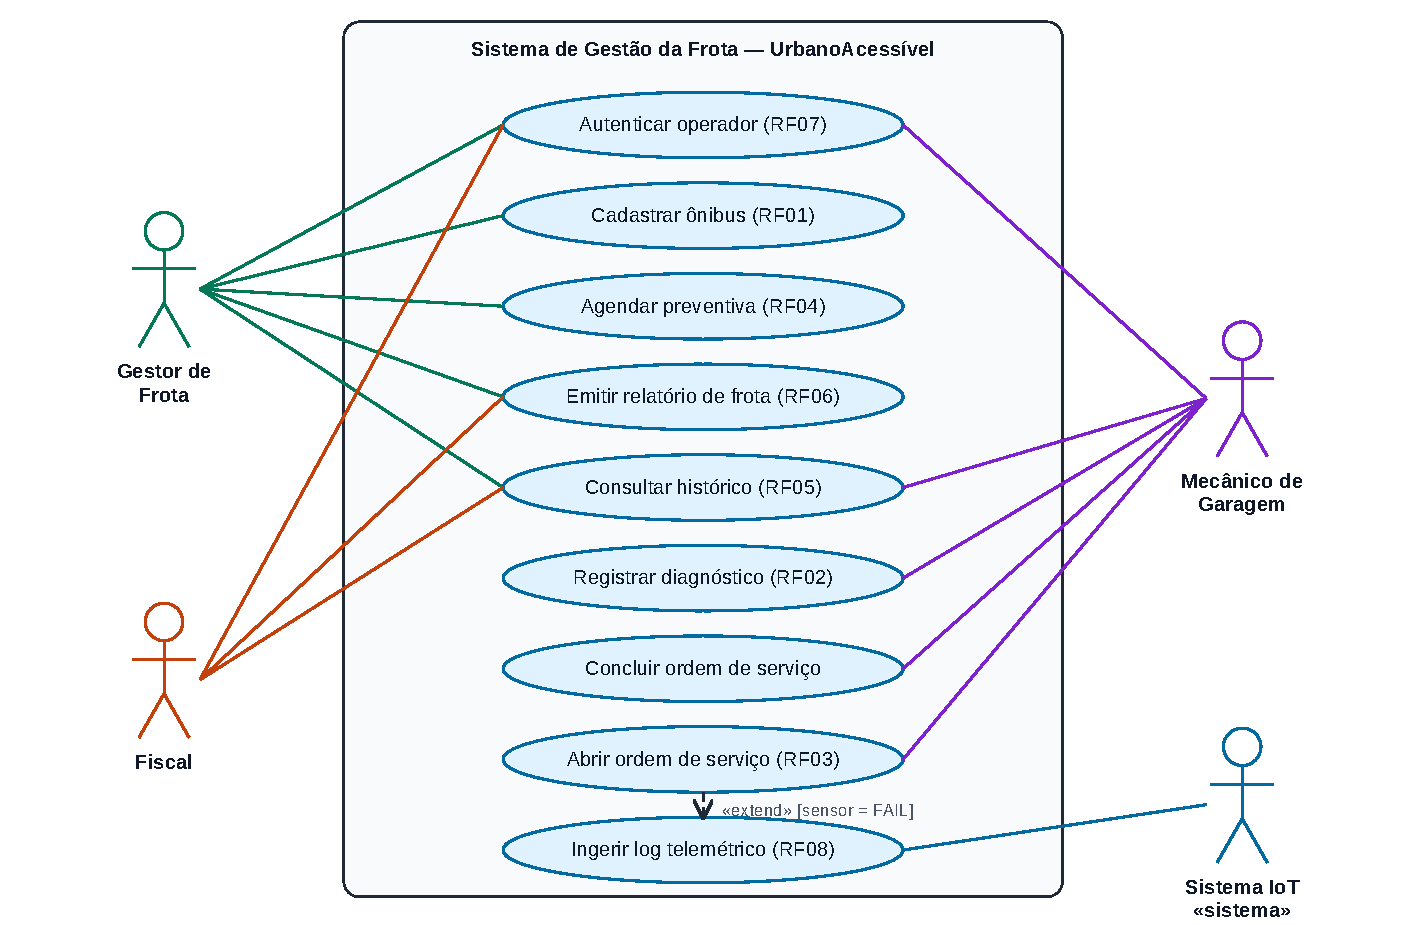
\includegraphics[width=0.92\textwidth]{fig/uc.pdf}
  \fonte{Elaborado pelo autor (2026).}
\end{figure}

A relação \guillemotleft extend\guillemotright{} entre ``Abrir ordem de serviço'' e ``Ingerir log
telemétrico'' indica que a abertura de OS é um comportamento opcional, acionado apenas quando a condição
\texttt{sensor = FAIL} é verdadeira. Todos os atores humanos passam pelo caso de uso de autenticação, que
determina o que cada perfil pode executar.

\section{Diagrama de classes}

O diagrama de classes da Figura~\ref{fig:classes} descreve as entidades do domínio e seus
relacionamentos. Como a implementação é em C, linguagem estruturada, cada classe foi mapeada para uma
estrutura (\texttt{struct}) e cada método para uma função que recebe um ponteiro para a estrutura. Os
atributos privados indicam que o acesso aos dados ocorre apenas por meio dessas funções, o que preserva o
encapsulamento mesmo sem suporte nativo da linguagem.

\begin{figure}[H]
  \centering
  \caption{Diagrama de classes}\label{fig:classes}
  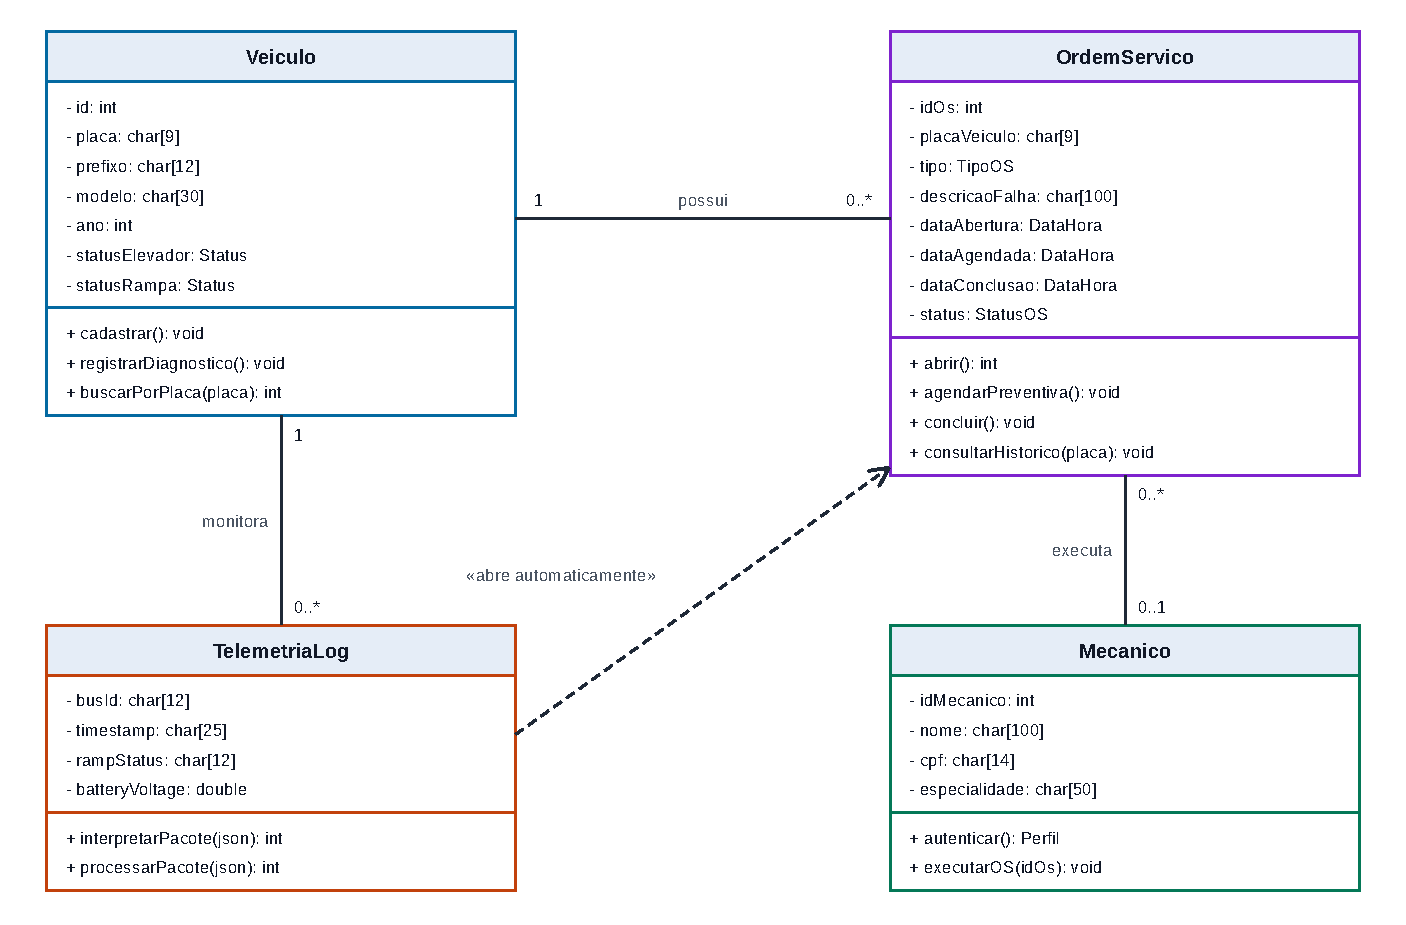
\includegraphics[width=0.92\textwidth]{fig/cl.pdf}
  \fonte{Elaborado pelo autor (2026).}
\end{figure}

Um \texttt{Veiculo} possui zero ou mais ordens de serviço e é monitorado por zero ou mais registros de
telemetria. Cada \texttt{OrdemServico} pode ser executada por no máximo um \texttt{Mecanico}; a
multiplicidade 0..1 do lado do mecânico reflete a decisão da retrospectiva da Sprint 1. A dependência
tracejada indica que \texttt{TelemetriaLog} pode criar uma \texttt{OrdemServico}.

\section{Diagrama de atividades}

O diagrama de atividades da Figura~\ref{fig:atividades} detalha, com raias, o fluxo mais crítico do
sistema: da falha do elevador até o veículo voltar ao estado operacional.

\begin{figure}[H]
  \centering
  \caption{Diagrama de atividades: da falha do elevador ao fechamento da OS}\label{fig:atividades}
  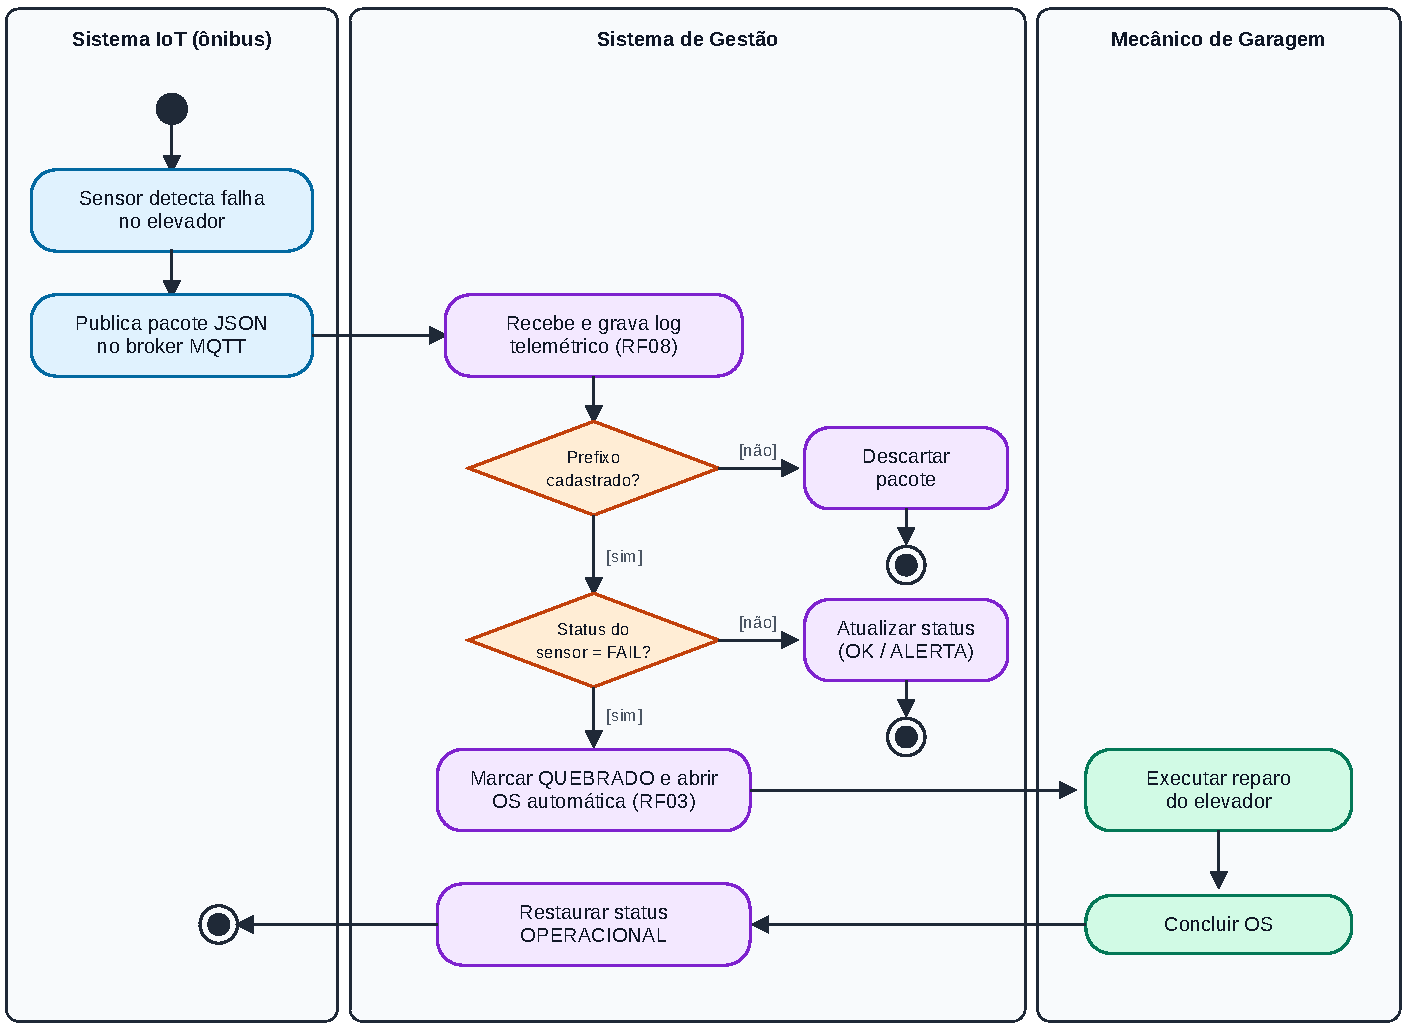
\includegraphics[width=0.86\textwidth]{fig/at.pdf}
  \fonte{Elaborado pelo autor (2026).}
\end{figure}

O sistema de gestão faz duas decisões. A primeira descarta pacotes de ônibus que não pertencem à frota
cadastrada, o que impede que um dispositivo desconhecido gere ordens. A segunda separa o estado de alerta
(\texttt{WARN}), que apenas atualiza o status do veículo, da falha (\texttt{FAIL}), que abre a ordem de
serviço. O mecânico executa o reparo e conclui a OS, e o sistema restaura o status para OPERACIONAL, o
que faz o veículo voltar a contar no indicador do RF06.

% =====================================================================
\chapter{BANCO DE DADOS RELACIONAL E NOSQL}\label{cap:bd}

\section{Persistência poliglota}

Os dados do sistema têm dois perfis distintos. Veículos, mecânicos e ordens de serviço são poucos,
estruturados, frequentemente cruzados em consultas e exigem integridade: uma OS não pode apontar para um
ônibus que não existe. Já a telemetria chega a cada cinco segundos de cada veículo, tem estrutura que
varia conforme a versão do firmware e raramente é alterada depois de gravada. \citeonline{sadalage}
chamam de persistência poliglota o uso de tecnologias de armazenamento diferentes para necessidades
diferentes dentro do mesmo sistema. Adotou-se, assim, um SGBD relacional (MySQL) para o domínio
transacional e um banco de documentos (MongoDB) para a telemetria.

\section{Modelo entidade-relacionamento}

A Figura~\ref{fig:der} apresenta o modelo lógico em notação de pé de galinha. Um veículo possui zero ou
muitas ordens de serviço, e cada ordem pertence obrigatoriamente a um veículo. Um mecânico executa zero
ou muitas ordens, e cada ordem tem no máximo um mecânico, pois a coluna \texttt{ID\_MECANICO} aceita valor
nulo.

\begin{figure}[H]
  \centering
  \caption{Diagrama entidade-relacionamento}\label{fig:der}
  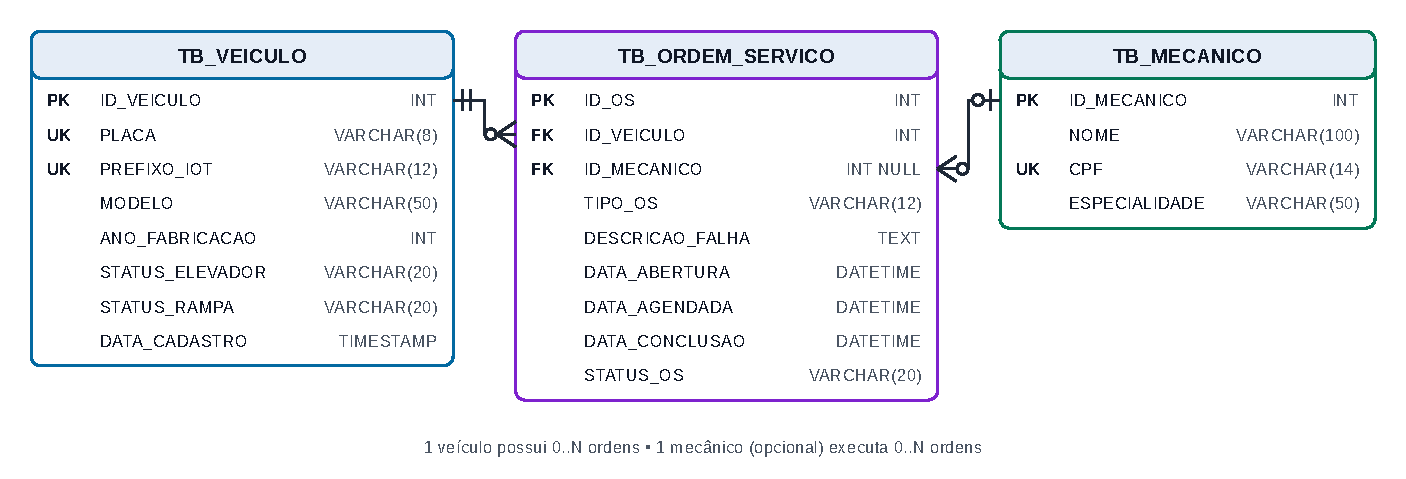
\includegraphics[width=0.95\textwidth]{fig/er.pdf}
  \fonte{Elaborado pelo autor (2026).}
\end{figure}

Em relação à especificação inicial, foram acrescentadas as colunas \texttt{PREFIXO\_IOT}, que liga o
veículo ao identificador enviado pelo sensor; \texttt{STATUS\_RAMPA}, para tratar rampa e elevador
separadamente; \texttt{TIPO\_OS} e \texttt{DATA\_AGENDADA}, que permitem registrar as manutenções
preventivas do RF04 na mesma tabela das corretivas.

\section{Normalização}

\citeonline{silberschatz} definem a normalização como um processo para obter esquemas que evitem
redundância desnecessária e anomalias de atualização. O modelo foi verificado em três etapas, sintetizadas
no Quadro~\ref{qd:normal}.

\begin{quadro}[H]
  \caption{Verificação das formas normais}\label{qd:normal}
  \small\singlespacing
  \renewcommand{\arraystretch}{1.25}
  \begin{tabularx}{\textwidth}{|>{\centering\arraybackslash}p{1.2cm}|>{\raggedright\arraybackslash}p{4.8cm}|X|}
    \hline
    \rowcolor{gray!15}\textbf{Forma} & \textbf{Regra} & \textbf{Aplicação no modelo} \\ \hline
    1FN & Todos os atributos têm valores atômicos, sem grupos repetidos. & O estado da acessibilidade foi dividido em \texttt{STATUS\_ELEVADOR} e \texttt{STATUS\_RAMPA}, em vez de um campo com lista. \\ \hline
    2FN & Está na 1FN e todo atributo não chave depende da chave primária inteira. & Todas as tabelas têm chave primária simples (\texttt{ID\_*}); não há dependência parcial possível. \\ \hline
    3FN & Está na 2FN e não há dependência transitiva entre atributos não chave. & O nome e a especialidade do mecânico ficam em \texttt{TB\_MECANICO}; a OS guarda apenas \texttt{ID\_MECANICO}. A placa não se repete na OS. \\ \hline
  \end{tabularx}
  \fonte{Elaborado pelo autor, com base em \citeonline{silberschatz} e \citeonline{elmasri}.}
\end{quadro}

\section{Scripts de definição de dados}

O Código~\ref{lst:ddl} cria as três tabelas. As restrições \texttt{CHECK} limitam os status aos valores
previstos, \texttt{UNIQUE} impede placas e prefixos duplicados, e as duas \texttt{FOREIGN KEY} garantem o
RNF04 no próprio SGBD.

\begin{lstlisting}[language=SQLm,caption={DDL das tabelas do sistema},label=lst:ddl]
CREATE TABLE TB_VEICULO (
    ID_VEICULO      INT AUTO_INCREMENT PRIMARY KEY,
    PLACA           VARCHAR(8)  NOT NULL UNIQUE,
    PREFIXO_IOT     VARCHAR(12) NOT NULL UNIQUE,
    MODELO          VARCHAR(50) NOT NULL,
    ANO_FABRICACAO  INT         NOT NULL,
    STATUS_ELEVADOR VARCHAR(20) DEFAULT 'OPERACIONAL',
    STATUS_RAMPA    VARCHAR(20) DEFAULT 'OPERACIONAL',
    DATA_CADASTRO   TIMESTAMP   DEFAULT CURRENT_TIMESTAMP,
    CHECK (STATUS_ELEVADOR IN ('OPERACIONAL','ALERTA','QUEBRADO')),
    CHECK (STATUS_RAMPA    IN ('OPERACIONAL','ALERTA','QUEBRADO'))
);
CREATE TABLE TB_MECANICO (
    ID_MECANICO   INT AUTO_INCREMENT PRIMARY KEY,
    NOME          VARCHAR(100) NOT NULL,
    CPF           VARCHAR(14)  NOT NULL UNIQUE,
    ESPECIALIDADE VARCHAR(50)  NOT NULL
);
CREATE TABLE TB_ORDEM_SERVICO (
    ID_OS           INT AUTO_INCREMENT PRIMARY KEY,
    ID_VEICULO      INT         NOT NULL,
    ID_MECANICO     INT         NULL,     -- OS automatica ainda sem responsavel
    TIPO_OS         VARCHAR(12) NOT NULL DEFAULT 'CORRETIVA',
    DESCRICAO_FALHA TEXT        NOT NULL,
    DATA_ABERTURA   DATETIME    NOT NULL,
    DATA_AGENDADA   DATETIME    NULL,
    DATA_CONCLUSAO  DATETIME    NULL,
    STATUS_OS       VARCHAR(20) DEFAULT 'EM_ABERTO',
    CHECK (TIPO_OS   IN ('CORRETIVA','PREVENTIVA')),
    CHECK (STATUS_OS IN ('EM_ABERTO','AGENDADA','CONCLUIDA')),
    FOREIGN KEY (ID_VEICULO)  REFERENCES TB_VEICULO(ID_VEICULO),
    FOREIGN KEY (ID_MECANICO) REFERENCES TB_MECANICO(ID_MECANICO)
);
CREATE INDEX IX_OS_STATUS ON TB_ORDEM_SERVICO (STATUS_OS, DATA_ABERTURA);
\end{lstlisting}
\fonte{Elaborado pelo autor (2026).}

\section{Consultas e manipulação de dados}

O Código~\ref{lst:dml} reúne as consultas que sustentam os requisitos de relatório. A primeira usa
\texttt{INNER JOIN} para listar as ordens em aberto com placa, modelo e mecânico. A segunda, do RF05, usa
\texttt{LEFT JOIN} para incluir também as ordens automáticas ainda sem mecânico, que um \texttt{INNER
JOIN} omitiria. A terceira calcula o indicador do RF06 com agregação condicional.

\begin{lstlisting}[language=SQLm,caption={Consultas com junções e indicador de frota},label=lst:dml]
-- Ordens em aberto com veiculo e mecanico
SELECT os.ID_OS, v.PLACA, v.MODELO, m.NOME AS MECANICO_RESPONSAVEL,
       os.DESCRICAO_FALHA, os.STATUS_OS, os.DATA_ABERTURA
FROM TB_ORDEM_SERVICO os
INNER JOIN TB_VEICULO  v ON os.ID_VEICULO  = v.ID_VEICULO
INNER JOIN TB_MECANICO m ON os.ID_MECANICO = m.ID_MECANICO
WHERE os.STATUS_OS = 'EM_ABERTO'
ORDER BY os.DATA_ABERTURA DESC;

-- RF05: historico de uma placa, inclusive OS sem mecanico
SELECT os.ID_OS, os.TIPO_OS, os.STATUS_OS, os.DATA_ABERTURA, os.DATA_CONCLUSAO,
       COALESCE(m.NOME, '(nao atribuido)') AS MECANICO
FROM TB_ORDEM_SERVICO os
INNER JOIN TB_VEICULO v ON os.ID_VEICULO = v.ID_VEICULO
LEFT  JOIN TB_MECANICO m ON os.ID_MECANICO = m.ID_MECANICO
WHERE v.PLACA = 'BRA2E19'
ORDER BY os.DATA_ABERTURA;

-- RF06: percentual da frota com acessibilidade 100% ativa
SELECT COUNT(*) AS TOTAL,
       ROUND(100.0 * SUM(CASE WHEN STATUS_ELEVADOR = 'OPERACIONAL'
                               AND STATUS_RAMPA    = 'OPERACIONAL'
                              THEN 1 ELSE 0 END) / COUNT(*), 1) AS PERCENTUAL_ATIVO
FROM TB_VEICULO;
\end{lstlisting}
\fonte{Elaborado pelo autor (2026).}

O fechamento de uma ordem corretiva altera duas tabelas: a OS passa a CONCLUIDA e o veículo volta a
OPERACIONAL. As duas instruções \texttt{UPDATE} foram agrupadas em uma transação
(\texttt{START TRANSACTION} \ldots{} \texttt{COMMIT}), de modo que uma falha entre elas não deixe o banco
em estado inconsistente. Os scripts foram executados em um banco de teste com dados de exemplo; as três
consultas retornaram os resultados esperados, e a inserção de uma OS para o veículo de código 99,
inexistente, foi recusada por violação de chave estrangeira.

\section{Modelo de documentos para a telemetria}

Cada ônibus envia um pacote a cada cinco segundos. Uma frota de quinhentos veículos operando dezoito horas
por dia gera cerca de 6,5 milhões de registros diários, volume para o qual uma tabela relacional com
índices e chaves estrangeiras seria um custo desnecessário. Os registros foram, então, modelados como
documentos JSON na coleção \texttt{telemetry\_logs} do MongoDB, conforme o Código~\ref{lst:json}.

\begin{lstlisting}[language=JSON,caption={Documento da coleção telemetry\_logs},label=lst:json,numbers=none]
{
  "_id": { "$oid": "673b5a1f8c9b1a2b3c4d5e6f" },
  "bus_id": "BUS-9042",
  "timestamp": { "$date": "2026-11-18T14:30:00Z" },
  "location": { "type": "Point", "coordinates": [-46.633308, -23.55052] },
  "accessibility_sensors": {
    "hydraulic_ramp_status": "OK",
    "tactile_floor_sensor": "OK",
    "wheelchair_bay_occupied": false
  },
  "passenger_load_pct": 62,
  "battery_voltage": 24.8,
  "firmware_version": "v2.1.4"
}
\end{lstlisting}
\fonte{Elaborado pelo autor (2026).}

Três decisões de projeto merecem registro. Primeiro, as coordenadas seguem o padrão GeoJSON, em que a
longitude vem antes da latitude; a versão preliminar do documento trazia a ordem invertida, o que faria o
índice geoespacial \texttt{2dsphere} posicionar o ônibus fora do mapa, e o erro foi corrigido. Segundo, foi
criado o índice composto \texttt{\{bus\_id: 1, timestamp: -1\}}, que localiza rapidamente a última leitura
de cada veículo. Terceiro, um índice TTL de 90 dias sobre \texttt{timestamp} faz o próprio banco expirar a
telemetria bruta \cite{mongodb}, aplicando o princípio da necessidade da LGPD, que limita o tratamento ao
mínimo necessário para a finalidade.

O documento não guarda dado pessoal: identifica o ônibus, nunca o passageiro ou o motorista. A ligação
entre os dois mundos é o prefixo IoT (\texttt{bus\_id}), presente tanto no documento quanto na coluna
\texttt{PREFIXO\_IOT} da tabela de veículos.

% =====================================================================
\chapter{PROGRAMAÇÃO EM C E PERSISTÊNCIA EM ARQUIVOS}\label{cap:c}

\section{Arquitetura modular}

O núcleo operacional do sistema foi escrito em C99, linguagem que, segundo
\citeonline{kernighan}, é de propósito geral e relativamente de baixo nível, adequada a programas em que
desempenho e controle de recursos importam. O código foi dividido em seis módulos, cada um com arquivo de
cabeçalho (\texttt{.h}) e implementação (\texttt{.c}), como mostra o Quadro~\ref{qd:modulos}.

\begin{quadro}[H]
  \caption{Módulos do programa em C}\label{qd:modulos}
  \small\singlespacing
  \renewcommand{\arraystretch}{1.25}
  \begin{tabularx}{\textwidth}{|>{\raggedright\arraybackslash}p{3.2cm}|X|>{\centering\arraybackslash}p{2.6cm}|}
    \hline
    \rowcolor{gray!15}\textbf{Módulo} & \textbf{Responsabilidade} & \textbf{Requisitos} \\ \hline
    \texttt{main.c} & Carrega os dados, autentica, exibe o menu e aplica a matriz de permissões. & RF07, RNF05 \\ \hline
    \texttt{veiculo.c} & Cadastro, diagnóstico, listagem, relatório e persistência da frota. & RF01, RF02, RF06 \\ \hline
    \texttt{ordem.c} & Abertura, agendamento, conclusão e histórico de ordens de serviço. & RF03--RF05, RNF04 \\ \hline
    \texttt{telemetria.c} & Interpretação do JSON, log telemétrico e abertura automática de OS. & RF03, RF08 \\ \hline
    \texttt{auth.c} & Operadores, hash de senha e perfis de acesso. & RF07 \\ \hline
    \texttt{util.c} & Leitura segura de texto e inteiros, data e hora, conversão de caixa. & RNF03, RNF05 \\ \hline
  \end{tabularx}
  \fonte{Elaborado pelo autor (2026).}
\end{quadro}

\section{Estruturas de dados}

O Código~\ref{lst:struct} apresenta as estruturas principais. Os vetores de caracteres têm tamanho igual ao
maior valor válido mais um byte para o terminador nulo; a placa no padrão Mercosul tem sete caracteres, e
o antigo, com hífen, oito, por isso \texttt{char placa[9]}. A estrutura \texttt{Frota} agrupa o vetor de
veículos, a quantidade cadastrada e o próximo identificador, e é declarada como variável estática em
\texttt{main.c}, fora da pilha, por ocupar cerca de 50 KB.

\begin{lstlisting}[language=C,caption={Estruturas Veiculo, Frota e OrdemServico},label=lst:struct]
typedef struct {
    int  id;
    char placa[9];            /* AAA0A00 ou AAA-0000 */
    char prefixo[12];         /* identificador IoT, ex.: BUS-9042 */
    char modelo[30];
    int  ano;
    char status_elevador[20]; /* OPERACIONAL, ALERTA, QUEBRADO */
    char status_rampa[20];
} Veiculo;

typedef struct {
    Veiculo itens[MAX_VEICULOS];
    int quantidade;
    int proximo_id;
} Frota;

typedef struct {
    int  id_os;
    char placa_veiculo[9];
    char tipo[12];                 /* CORRETIVA, PREVENTIVA */
    char descricao_falha[100];
    char data_abertura[TAM_DATA];
    char data_agendada[TAM_DATA];  /* "-" quando nao se aplica */
    char data_conclusao[TAM_DATA]; /* "-" enquanto aberta */
    char status[15];               /* EM_ABERTO, AGENDADA, CONCLUIDA */
} OrdemServico;
\end{lstlisting}
\fonte{Elaborado pelo autor (2026).}

\section{Persistência em arquivo}

Cada entidade é gravada em um arquivo de texto, uma linha por registro, com campos separados por
ponto e vírgula, formato legível que pode ser aberto em qualquer editor ou importado por uma planilha. Ao
iniciar, o programa lê os arquivos para a memória; a cada alteração, regrava o arquivo inteiro.

A especificação preliminar gravava os veículos com \texttt{fopen} em modo de acréscimo e os lia com
\texttt{fscanf} em um laço encerrado apenas por \texttt{EOF}. Essa abordagem tem dois problemas. O modo de
acréscimo não permite alterar um registro já gravado, e o RF02 precisa mudar o status do elevador; e, se
uma linha estiver corrompida, \texttt{fscanf} deixa de consumir a entrada sem atingir o fim do arquivo, e
o laço nunca termina. A versão final, no Código~\ref{lst:persist}, lê cada linha com \texttt{fgets} e
confere quantos campos \texttt{sscanf} converteu, descartando linhas inválidas.

\begin{lstlisting}[language=C,caption={Leitura e gravação atômica da frota},label=lst:persist]
int carregarFrota(Frota *f) {
    FILE *arq;
    char linha[256];
    f->quantidade = 0;
    f->proximo_id = 1;
    arq = fopen(ARQ_FROTA, "r");
    if (arq == NULL) return 0;   /* primeira execucao */
    while (fgets(linha, sizeof linha, arq) != NULL && f->quantidade < MAX_VEICULOS) {
        Veiculo v;
        int lidos = sscanf(linha, "%d;%8[^;];%11[^;];%29[^;];%d;%19[^;];%19[^\r\n]",
                           &v.id, v.placa, v.prefixo, v.modelo, &v.ano,
                           v.status_elevador, v.status_rampa);
        if (lidos == 7) {        /* linha corrompida nao trava o laco */
            f->itens[f->quantidade++] = v;
            if (v.id >= f->proximo_id) f->proximo_id = v.id + 1;
        }
    }
    fclose(arq);
    return f->quantidade;
}

int salvarFrota(const Frota *f) {
    const char *tmp = ARQ_FROTA ".tmp";
    FILE *arq = fopen(tmp, "w");
    int i;
    if (arq == NULL) return 0;
    for (i = 0; i < f->quantidade; i++) {
        const Veiculo *v = &f->itens[i];
        fprintf(arq, "%d;%s;%s;%s;%d;%s;%s\n", v->id, v->placa, v->prefixo,
                v->modelo, v->ano, v->status_elevador, v->status_rampa);
    }
    if (fclose(arq) != 0) return 0;
    remove(ARQ_FROTA);
    return rename(tmp, ARQ_FROTA) == 0;
}
\end{lstlisting}
\fonte{Elaborado pelo autor (2026).}

A gravação é feita primeiro em um arquivo temporário e só depois o original é substituído com
\texttt{rename}. Se o programa for interrompido no meio da escrita, o arquivo anterior continua íntegro,
o que atende ao RNF02. Os especificadores de largura em \texttt{sscanf}, como \texttt{\%8[\textasciicircum;]},
impedem que um campo maior que o esperado ultrapasse o tamanho do vetor. Para o mesmo fim, a entrada do
teclado é lida com \texttt{fgets} na função \texttt{lerTexto()}, e não com \texttt{scanf("\%s")}, que não
limita o tamanho; a função também recusa o caractere ponto e vírgula, reservado como separador.

\section{Integridade referencial e abertura automática de OS}

O Código~\ref{lst:abrir} mostra o núcleo da abertura de ordens, compartilhado pela abertura manual (RF03),
pelo agendamento de preventivas (RF04) e pela abertura automática via telemetria. Antes de criar a OS, a
função procura a placa na frota; se não encontrar, recusa a operação. É o equivalente, em arquivo, à
chave estrangeira do banco relacional. Se a gravação em disco falhar, a inserção em memória é desfeita,
mantendo memória e arquivo sincronizados.

\begin{lstlisting}[language=C,caption={Abertura de OS com verificação de integridade},label=lst:abrir]
int abrirOrdem(CadastroOS *c, const Frota *f, const char *placa,
               const char *tipo, const char *descricao, const char *data_agendada) {
    OrdemServico o;
    if (buscarVeiculoPorPlaca(f, placa) < 0) {
        printf("  [RNF04] Recusado: veiculo %s nao existe na frota.\n", placa);
        return 0;
    }
    o.id_os = c->proximo_id;
    /* ... copia dos campos com strncpy e terminador garantido ... */
    dataHoraAtual(o.data_abertura, sizeof o.data_abertura);
    strcpy(o.data_agendada, data_agendada ? data_agendada : "-");
    strcpy(o.data_conclusao, "-");
    strcpy(o.status, data_agendada ? "AGENDADA" : "EM_ABERTO");
    c->itens[c->quantidade++] = o;
    if (!salvarOrdens(c)) { c->quantidade--; return 0; }
    return c->proximo_id++;
}
\end{lstlisting}
\fonte{Elaborado pelo autor (2026).}

A ingestão de telemetria (RF08) lê um arquivo no formato JSON Lines, um pacote por linha, exportado pelo
broker. Para cada pacote, o programa extrai \texttt{bus\_id} e \texttt{hydraulic\_ramp\_status}, grava o
registro em \texttt{telemetria\_log.txt} e atualiza o veículo correspondente. Um status \texttt{WARN} muda
o elevador para ALERTA; um status \texttt{FAIL} o muda para QUEBRADO e abre a OS, desde que não exista
outra ordem corretiva em aberto para o mesmo ônibus. Essa última verificação é necessária porque o sensor
repete a falha a cada cinco segundos, e sem ela um único defeito geraria centenas de chamados. O
interpretador de JSON foi escrito de forma simples, por busca de chave, suficiente para o pacote plano do
sensor; em produção, recomenda-se uma biblioteca dedicada.

\section{Controle de acesso por perfil}

Os operadores ficam em \texttt{operadores.txt}, criado na primeira execução com três contas padrão,
exibidas na tela nesse momento e documentadas no arquivo \texttt{README.md}: \texttt{gestor} (senha
\texttt{gestor123}), \texttt{mecanico} (senha \texttt{mec123}) e \texttt{fiscal} (senha
\texttt{fiscal123}). Para restaurá-las, basta apagar o arquivo. As
senhas não são gravadas em texto puro, mas como resumo pela função de hash djb2, limitado a 32 bits para
produzir o mesmo valor no Windows, em que \texttt{unsigned long} tem 32 bits, e no Linux, em que tem 64.
O djb2 não é um algoritmo criptográfico; foi usado por fins didáticos, e um sistema real deve usar
bcrypt ou Argon2 com sal. Após três tentativas inválidas o acesso é bloqueado. A função
\texttt{permitido()} implementa a matriz de permissões: apenas o Gestor cadastra veículos e importa
telemetria; Gestor e Mecânico registram diagnósticos e movimentam ordens; o Fiscal tem acesso somente às
consultas e relatórios.

\section{Testes e resultados}

Os testes foram realizados com roteiros de entrada redirecionados ao programa, o que permite repeti-los a
cada alteração. O Quadro~\ref{qd:testes} resume os casos executados.

\begin{quadro}[H]
  \caption{Casos de teste executados}\label{qd:testes}
  \small\singlespacing
  \renewcommand{\arraystretch}{1.25}
  \begin{tabularx}{\textwidth}{|>{\centering\arraybackslash}p{0.9cm}|X|X|>{\centering\arraybackslash}p{1.6cm}|}
    \hline
    \rowcolor{gray!15}\textbf{N.º} & \textbf{Entrada} & \textbf{Resultado obtido} & \textbf{Situação} \\ \hline
    1 & Senha incorreta seguida da correta & Mensagem com tentativas restantes; acesso concedido na segunda & Aprovado \\ \hline
    2 & Cadastro de BRA2E19 e FIX3D45 & Veículos com ID 1 e 2 gravados no arquivo & Aprovado \\ \hline
    3 & Novo cadastro com placa BRA2E19 & Recusado: placa duplicada & Aprovado \\ \hline
    4 & Opção de menu ``12'' & Mensagem de valor inválido e nova leitura & Aprovado \\ \hline
    5 & OS para a placa XYZ9999 & Recusada com aviso RNF04 & Aprovado \\ \hline
    6 & Importação de 5 pacotes IoT (OK, WARN, FAIL, FAIL, prefixo desconhecido) & 4 pacotes gravados, 1 OS automática, nenhuma duplicada, 1 ignorado & Aprovado \\ \hline
    7 & Relatório de frota após a importação & 0\% ativa, 50\% em alerta, 50\% quebrada & Aprovado \\ \hline
    8 & Conclusão da OS automática & OS concluída; frota passa a 50\% ativa & Aprovado \\ \hline
    9 & Reinício do programa com perfil Fiscal & Dados recarregados; cadastro bloqueado pelo perfil & Aprovado \\ \hline
    10 & Compilação com \texttt{-std=c99 -Wall -Wextra -pedantic} & Nenhum aviso ou erro & Aprovado \\ \hline
  \end{tabularx}
  \fonte{Elaborado pelo autor (2026).}
\end{quadro}

O Código~\ref{lst:saida} reproduz um trecho da saída real do programa durante os casos de teste 6 e 7,
mostrando a abertura automática da OS e o cálculo do indicador do RF06.

\begin{lstlisting}[caption={Trecho da execução do programa},label=lst:saida,numbers=none,basicstyle=\ttfamily\scriptsize\linespread{1}\selectfont]
=== RF08 - INGESTAO DE LOG TELEMETRICO ===
  BUS-9042 (BRA2E19): sensores OK.
  BUS-7110 (FIX3D45): status ALERTA registrado.
  BUS-9042 (BRA2E19): FALHA! OS automatica #1 aberta.
  BUS-9042 (BRA2E19): status QUEBRADO registrado.
  [!] BUS-0001 nao pertence a frota cadastrada. Pacote ignorado.
>> 4 pacote(s) gravados em telemetria_log.txt; 1 OS automatica(s).

=== RF06 - RELATORIO DE FROTA OPERACIONAL ===
Total de veiculos ........: 2
Acessibilidade 100% ativa : 0 (0.0%)
Em alerta ................: 1 (50.0%)
Com equipamento quebrado .: 1 (50.0%)
\end{lstlisting}
\fonte{Elaborado pelo autor (2026).}

\section{Compilação, portabilidade e integração com a plataforma web}

O programa usa apenas a biblioteca padrão do C (\texttt{stdio.h}, \texttt{stdlib.h}, \texttt{string.h},
\texttt{ctype.h} e \texttt{time.h}), sem chamadas de sistema como \texttt{system("cls")} ou
\texttt{conio.h}, o que atende ao RNF03 \cite{iso9899}. Em Linux, a compilação é feita com o
\texttt{Makefile} fornecido ou com \texttt{gcc -std=c99 -Wall -Wextra -o urbano src/*.c}; no Windows, o
mesmo comando funciona no terminal do MinGW, gerando \texttt{urbano.exe}. Os arquivos de dados são
criados na pasta em que o programa é executado.

Para apresentar a jornada do PIM III ao PIM IV, foi desenvolvida também uma plataforma web em HTML, CSS e
JavaScript, com tema escuro, animações GSAP acionadas pela rolagem e efeito parallax. Ela reúne a
topologia interativa, a tradução didática dos comandos Cisco, os diagramas UML, os scripts de banco de
dados e um terminal que simula a execução do programa em C, com os mesmos menus e validações, exibindo os
arquivos em disco sendo atualizados. A plataforma segue as próprias diretrizes do projeto: navegação por
teclado, alto contraste, ajuste do tamanho do texto e opção de reduzir as animações.

% =====================================================================
\chapter{CONCLUSÃO}\label{cap:conclusao}

Este trabalho desenvolveu o Sistema Corporativo de Gestão da Frota, Manutenção Preventiva e Chamados de
Acessibilidade da UrbanoAcessível S.A., dando sequência à infraestrutura de redes e nuvem projetada no
PIM III. Os objetivos propostos foram atingidos: os oito requisitos funcionais e os cinco não funcionais
foram levantados, distribuídos em três sprints e modelados em diagramas UML; o banco relacional foi
normalizado até a terceira forma normal e complementado por uma coleção de documentos para a telemetria;
e o programa em C implementou todas as funcionalidades, com persistência em disco verificada nos testes.

A integração entre as disciplinas mostrou-se o ponto mais instrutivo do projeto. A mesma regra de
negócio, a de que não existe ordem de serviço sem veículo, apareceu no diagrama de classes como
multiplicidade, no banco como chave estrangeira e no código como uma busca antes da inserção. Também
ficou claro que a escolha da tecnologia de armazenamento depende do perfil do dado: o relacional para o
que exige integridade, o documental para o que chega em grande volume e muda de formato.

Durante o desenvolvimento, a especificação preliminar foi revisada em três pontos: a leitura de arquivo
com laço que poderia não terminar, o modo de gravação que impedia atualizar registros e a ordem das
coordenadas no documento GeoJSON. Essas correções reforçam a importância dos testes e da revisão contínua
previstos no processo ágil.

Como limitações, o programa em C mantém os dados em vetores de tamanho fixo e reescreve o arquivo inteiro a
cada alteração, abordagem adequada a uma garagem, mas não a uma frota metropolitana inteira. O hash de
senha é didático e o interpretador de JSON é restrito ao formato do sensor. Como trabalhos futuros,
sugerem-se a conexão do programa ao MySQL por meio da biblioteca cliente, a assinatura direta do tópico
MQTT, em vez da leitura de arquivo exportado, e um aplicativo para o passageiro que informe qual o próximo
ônibus com elevador funcionando no seu ponto.

Por fim, o indicador de frota acessível do RF06 transforma um direito previsto em lei em um número
verificável. É nesse ponto que a tecnologia deixa de ser apenas infraestrutura e passa a servir à
inclusão das pessoas que mais dependem do transporte público.

% =====================================================================
%  REFERÊNCIAS (NBR 6023:2018)
% =====================================================================
\clearpage
\phantomsection
\addcontentsline{toc}{chapter}{\MakeUppercase{Referências}}
\titulocentral{Referências}
{\singlespacing\raggedright
\setlength{\parindent}{0pt}
\setlength{\parskip}{\baselineskip}

BECK, Kent. \textbf{Programação extrema (XP) explicada}: acolha as mudanças. Porto Alegre: Bookman, 2004.

BRASIL. [Constituição (1988)]. \textbf{Constituição da República Federativa do Brasil de 1988}.
Brasília, DF: Presidência da República, 1988. Disponível em:
http://www.planalto.gov.br/ccivil\_03/constituicao/constituicao.htm. Acesso em: 18 nov. 2026.

BRASIL. Lei nº 13.146, de 6 de julho de 2015. Institui a Lei Brasileira de Inclusão da Pessoa com
Deficiência (Estatuto da Pessoa com Deficiência). \textbf{Diário Oficial da União}: seção 1, Brasília,
DF, 7 jul. 2015.

BRASIL. Lei nº 13.709, de 14 de agosto de 2018. Lei Geral de Proteção de Dados Pessoais (LGPD).
\textbf{Diário Oficial da União}: seção 1, Brasília, DF, 15 ago. 2018.

ELMASRI, Ramez; NAVATHE, Shamkant B. \textbf{Sistemas de banco de dados}. 7. ed. São Paulo: Pearson,
2018.

FOWLER, Martin. \textbf{UML essencial}: um breve guia para a linguagem padrão de modelagem de objetos.
3. ed. Porto Alegre: Bookman, 2005.

GIL, Antonio Carlos. \textbf{Como elaborar projetos de pesquisa}. 6. ed. São Paulo: Atlas, 2017.

INTERNATIONAL ORGANIZATION FOR STANDARDIZATION. \textbf{ISO/IEC 9899:1999}: programming languages -- C.
Geneva: ISO, 1999.

KERNIGHAN, Brian W.; RITCHIE, Dennis M. \textbf{C}: a linguagem de programação padrão ANSI. Rio de
Janeiro: Campus, 1989.

LAKATOS, Eva Maria; MARCONI, Marina de Andrade. \textbf{Fundamentos de metodologia científica}. 8. ed.
São Paulo: Atlas, 2017.

MONGODB, INC. \textbf{MongoDB Manual}: TTL indexes. [\textit{S. l.}]: MongoDB, 2026. Disponível em:
https://www.mongodb.com/docs/manual/core/index-ttl/. Acesso em: 18 nov. 2026.

PRESSMAN, Roger S.; MAXIM, Bruce R. \textbf{Engenharia de software}: uma abordagem profissional. 8. ed.
Porto Alegre: AMGH, 2016.

SADALAGE, Pramod J.; FOWLER, Martin. \textbf{NoSQL essencial}: um guia conciso para o mundo emergente da
persistência poliglota. São Paulo: Novatec, 2013.

SCHWABER, Ken; SUTHERLAND, Jeff. \textbf{O guia do Scrum}: o guia definitivo para o Scrum: as regras do
jogo. [\textit{S. l.}]: Scrum.org, 2020. Disponível em: https://scrumguides.org. Acesso em: 18 nov. 2026.

SILBERSCHATZ, Abraham; KORTH, Henry F.; SUDARSHAN, S. \textbf{Sistema de banco de dados}. 6. ed. Rio de
Janeiro: Elsevier, 2012.

SOMMERVILLE, Ian. \textbf{Engenharia de software}. 10. ed. São Paulo: Pearson, 2018.

TANENBAUM, Andrew S.; WETHERALL, David. \textbf{Redes de computadores}. 5. ed. São Paulo: Pearson, 2011.

W3C. \textbf{Web Content Accessibility Guidelines (WCAG) 2.1}. [\textit{S. l.}]: W3C, 2018. Disponível
em: https://www.w3.org/TR/WCAG21/. Acesso em: 18 nov. 2026.
\par}

% =====================================================================
%  APÊNDICES
% =====================================================================
\clearpage
\phantomsection
\addcontentsline{toc}{chapter}{\MakeUppercase{Apêndice A -- Código-fonte completo do programa em C}}
\titulocentral{Apêndice A -- Código-fonte completo do programa em C}

\lstset{basicstyle=\ttfamily\scriptsize\linespread{1}\selectfont}
\lstinputlisting[language=C,title={\small\texttt{src/main.c}},nolol]{../programa_c/src/main.c}
\lstinputlisting[language=C,title={\small\texttt{src/util.h}},nolol]{../programa_c/src/util.h}
\lstinputlisting[language=C,title={\small\texttt{src/util.c}},nolol]{../programa_c/src/util.c}
\lstinputlisting[language=C,title={\small\texttt{src/veiculo.h}},nolol]{../programa_c/src/veiculo.h}
\lstinputlisting[language=C,title={\small\texttt{src/veiculo.c}},nolol]{../programa_c/src/veiculo.c}
\lstinputlisting[language=C,title={\small\texttt{src/ordem.h}},nolol]{../programa_c/src/ordem.h}
\lstinputlisting[language=C,title={\small\texttt{src/ordem.c}},nolol]{../programa_c/src/ordem.c}
\lstinputlisting[language=C,title={\small\texttt{src/telemetria.h}},nolol]{../programa_c/src/telemetria.h}
\lstinputlisting[language=C,title={\small\texttt{src/telemetria.c}},nolol]{../programa_c/src/telemetria.c}
\lstinputlisting[language=C,title={\small\texttt{src/auth.h}},nolol]{../programa_c/src/auth.h}
\lstinputlisting[language=C,title={\small\texttt{src/auth.c}},nolol]{../programa_c/src/auth.c}

\end{document}
